% ------------------------------------------------------------
\section{Calendar Week}
% ------------------------------------------------------------
% --------------------------------------------------- Slide --
\subsection{CW 29}
% ------------------------------------------------------------
\begin{frame}
  \frametitle{Review CW 29}
	\begin{itemize}
		\item Inquiry regarding "Remote Access" -> Answer from IT: It can take a while... - \textcolor{yellow}{In Work} 
		\item Add possibility of multi-steps to created script. Objective: calculate and accumulate damage due to different loads in a single run of the script. - \textcolor{yellow}{In Work} 
		\item Further papers read this week: Irandoust2020, Velasco-Ortega2019, Jafarian2019, Korabi2017. - \textcolor{green}{Done}
	\end{itemize}
\end{frame}

\begin{frame}
	\frametitle{Papers Read - CW29}
	\begin{figure}
	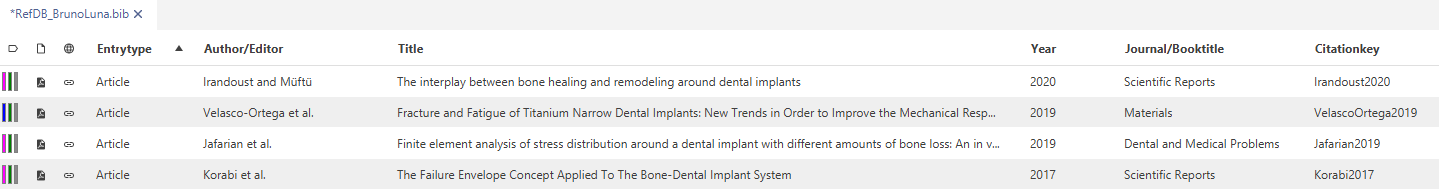
\includegraphics[width=1.0\textwidth]{pictures/CW29_1}
	\caption{Screen capture from JabRef.}
	\end{figure}
\end{frame}

% ------------------------------------------------------------
% --------------------------------------------------- Slide --
\subsection{CW 30}
% ------------------------------------------------------------
% ------------------------------------------------------------
\begin{frame}
  \frametitle{Outlook CW 30}
	\begin{itemize}
		\item Continue work on adding possibility of multi-steps to created script. Objective: calculate and accumulate damage due to different loads in a single run of the script.
	\end{itemize}
\end{frame}
% --------------------------------------------------- Slide --

